\section{Contribution}
The goal of this work is to discuss a complementary approach to current operations based on an experiment-agnostic, computer-aided strategy to grid monitoring centered on error messages rather than site performances.

In particular, we propose an unsupervised Machine Learning (ML) pipeline to identify clusters of similar failures. These groups of errors retrieved in this way are then exposed to shifters as suggestions of potential issues to investigate further.

\begin{landscape}
\begin{figure}
    \centering
    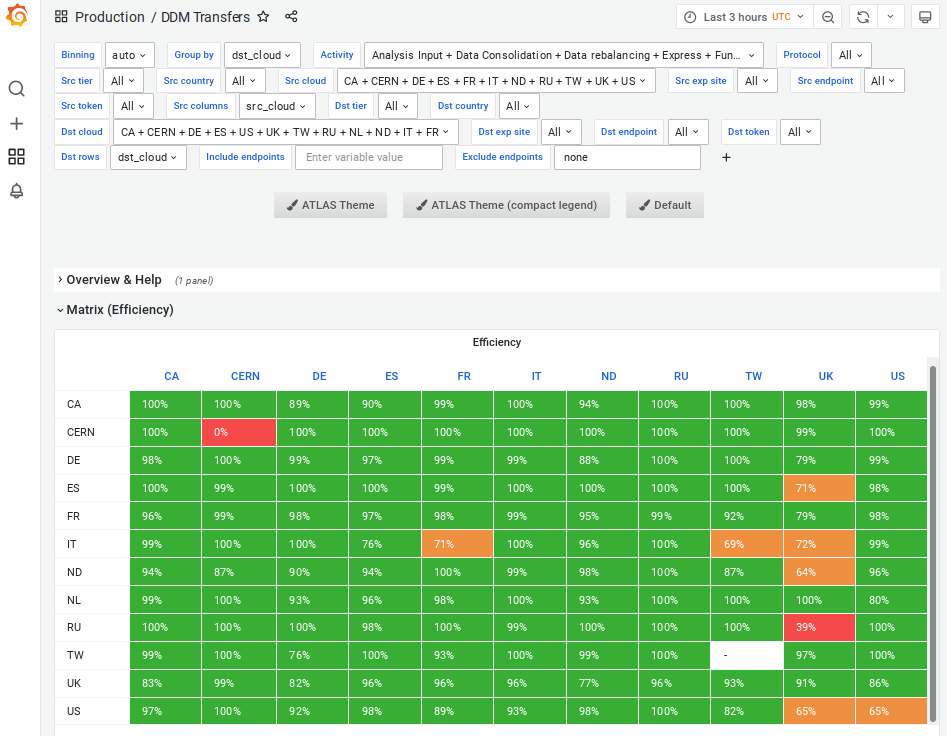
\includegraphics[height=\textwidth]{figures/220_introduction/grafana_efficiency_matrix_narrow1.png}
    \caption{Transfer efficiency matrix from Grafana. Transfer sources are shown as columns and destinations as rows. The drop-down menus at the top allow for custom filtering at the desired level of granularity.}
    \label{fig:efficiency_matrix}
\end{figure}
\end{landscape}
